% \setchapterimage[6cm]{seaside}
\setchapterstyle{kao}
\setchapterpreamble[u]{\margintoc}
\chapter{The first large language model for French}
% using a generative objective
\labch{generative}

\cleanchapterquote{Le sujet s'éloigne du verbe... et le complément direct vient se poser quelque part dans le vide.}{Samuel Beckett}{En attendant Godot, 1953}

% \section{Training efficient sentence embedding models using structured encoders}
% \labsec{structure-scale}
In the previous sections, we explored the training of models by predicting the relations between sentences. In this case, we are mining a specific datasets with many sentence pairs. There are also methods for reconstructing a noised input, for example detecting masked words or predicting what the next word will be. The corpora required for such auto-encoding methods are more simple and only consist in individual documents.

In this section, we introduce a French adaptation from the well-known GPT model. GPT relies on transformer pre-trained architectures, which profoundly transformed natural language processing methods. Such models are pre-trained using a self-supervised objective and are therefore specific to a given language. The model, equivalent to GPT-2 in English, contains more than 1 billion parameters. This work benefited from access to the IDRIS computing facilities through the allocation of 2020-AD011011823 allocated by GENCI.

Even though the pre-training objective is relatively simple, deep neural networks may acquire shocking grammar abilities \parencite{linzen_2020}. For example, GPT-2 generates correct text with plural and long-distance agreement despite any prior linguistic knowledge. Such agreements are determined by abstract structures and not just linear order of words. Surprisingly, models can learn such specific linguistic patterns (subject-verb, noun-adverb, verb-verb) with no prior information about linguistic theory. 

Although some models may exist in French, the majority is released in English only. The model can address a large variety of tasks. In particular, the model may benefit from original configurations such as few-shot or zero-shot learning. In such configurations, it is possible to address tasks without any parameters fine-tuning. We organize the section as follow: We first present the construction of the training and evaluation corpora (\refsec{generative:corpus}). We then detail the architecture and training setup in \refsec{generative:models}. Finally,  \refsec{generative:evaluation} examines our model abilities through several evaluation tests.
%GPT achieves impressive language generation performances. 

% Within my laboratory, I led the project to train the first large language model in French \parencite{simoulin_2021c}. We obtained a dedicated computation grant on public French HPC computer Jean Zay. The model, equivalent to GPT-2 in English, contains more than 1 billion parameters. We built a dedicated training corpus and parallelized the training between multiple nodes and compute units. I am particularly proud of this project, as we contributed to the resources available in French. We released the model in Open-Source for research and business application purposes. 

%TODO il faut parler des embeddings de phrase de ces modèles et le relier à la problématique de la thèse

\section{Introduction}
\labsec{generative:introduction}

Pre-trained generative models leverage the generative properties of language models by employing an alternative training and inference paradigm \parencite{radford_2018, radford_2019, brown_20}. With this paradigm, the model directly generates the answer in natural language, allowing them to accomplish a variety of tasks without changing the architecture. Fhurthermore, this setup doesn’t require to fine-tune the model weights on examples specific to the task. Instead, the model outputs are conditioned by controlling the input feed to the model, or "prompt". Usually, the prompt includes a brief description of the task and examples formatted as a sequential completion task. This setup can be extended to a zero-shot learning configuration, for which the prompt only contains the description of the task and the examples to be inferred.

Still, the generality of what are sometimes called "foundation" models has some limitations. First, the pre-training is specific to a given language, and extending it to other languages is not trivial. It requires large corpora of raw text—up to billion of tokens. Second, pre-training also requires significant computing power, typically dozens of GPUs or TPUs\sidenote{\url{https://cloud.google.com/tpu}} operating for several days. Last but not least, the analysis and evaluation of these models requires access to relevant and rigorous benchmarks.

This is, to the best of our knowledge, the first peer-reviewed contribution that adapts pre-trained generative transformers to French. We adapt OpenAI GPT et GPT-2 \parencite{radford_2018, radford_2019} for French. Our contributions are the following:
\begin{itemize}
    \item We propose a corpus dedicated to the training of transformers language models in French. The construction of thus corpus is detailed in \refsec{generative:corpus} ;
    \item We developed two models with a large number of parameters, which we released as open-source contributions\sidenote{\url{https://huggingface.co/asi/gpt-fr-cased-base}}. Hopefully, these models can be used in academic as well as industrial settings. We detailed the architecture of the models in \refsec{generative:models} ;
    \item We replicate English evaluation benchmarks for French language models. This evaluation setup allows for the comparison of models and is detailed in \refsec{generative:evaluation}.
\end{itemize}

\section{Building the corpora}
\labsec{generative:corpus}

\paragraph{Pre-training corpus} For pre-training, generative transformers require only raw text. However, training such models requires large corpora due to their large number of parameters. Documents used for GPT model training are typically much longer than those used for \textsc{Bert} \parencite{devlin_19}. The majority of the corpora used to adapt \textsc{Bert} in French: Camembert \parencite{martin_20} or Flaubert \parencite{le_20b, le_20a} use relatively short documents for which the sequential order of between chunks in not preserved. Because of this, we couldn't use them directly and build our own corpus. We instead aggregated two training corpora with different scales to train our models. We summarize their main statistics in \reftab{generative:corpus-size}.

\begin{table}[!htbp]
\centering
    \begin{tabularx}{\textwidth}{l|YYYY}
    Models & OpenAI GPT &  OpenAI GPT-2 & $\text{GPT}_{fr}$-124M & $\text{GPT}_{fr}$-1B \\\hline
    % Modèles & Nombre de documents ($\times 10^6$) & Nombre de mots ($\times 10^9$)
    % OpenAI GPT & 2,262,211$^\dagger$ & 1,158,252,402$^\dagger$   \\
    % OpenAI GPT-2 & 8,000,000 & 4,680,000,000$^\dagger$ \\
    % Fr GPT-124M & 1,656,080 & 1,597,377,426 \\
    % Fr GPT-1B & 7,356,862 & 3,106,521,195
    \# Documents ($\times 10^6$) & 2,26$^\dagger$ & 8,00 & 1,66 & 7,36 \\
    \# Tokens ($\times 10^9$)& 1,16$^\dagger$ & 4,68$^\dagger$ & 1,60 & 3,11\\
    Avg. tokens per document & \numprint{512}$^\dagger$ & \numprint{585}$^\dagger$ & \numprint{965} & \numprint{422}
    \end{tabularx}
\caption{\labtab{generative:corpus-size}
 Statistics of the corpora used to pre-train the models. The $\dagger$ denote estimates based on the available data. Specifically, we hypothesize that the number of tokens per document is equal to the context size for OpenAI GPT. We estimate the OpenAI GPT-2 statistics using the open-source sample: \url{https://github.com/openai/gpt-2-output-dataset}.}
\end{table}

We create a first corpus, used to train the first model $\text{GPT}_{fr}$-124M, is an aggregation of existing corpora: Wikipedia\sidenote{\url{https://dumps.wikimedia.org/frwiki/}}, OpenSubtitle\sidenote{\url{http://opus.nlpl.eu/download.php?f=OpenSubtitles/v2016/mono/}} \parencite{tiedemann_12} and Gutenberg\sidenote{\url{http://www.gutenberg.org}}. We divide documents into successive sentences and concatenate them into documents of maximum \numprint{1024} tokens. 

We then create a second corpus to train our model with above 1 billion parameters: $\text{GPT}_{fr}$-1B. Our approach is to augment the first corpus with data from the Common Crawl\sidenote{\url{http://data.statmt.org/ngrams/deduped2017/}} in French. Taking inspiration from the procedure outlined in \textcite{brown_20}, we filter the Common Crawl data in several steps. First, we exclude all the documents too short with less than 128 tokens, as done in \textcite{shoeybi_19}. We filtered out 93\% of the raw documents using this very simple filter. We then filter out documents whose word distribution differed too much from the first corpus. By using \numprint{200000}  randomly chosen documents, we train a binary classifier to discriminate between documents in the first corpus and those in the Common Crawl. We excluded all documents that had a probability <10\% to be extracted from the first corpus. The filter, deliberately unselective, is designed to filter out explicitly invalid or poorly formatted documents. Finally we apply a filter targeting the structure of documents. We selected documents with a low perplexity\sidenote{Given a sequence $U=\{u_1 \cdots u_n\}$, we define the perplexity as: $PPL(U) = exp \left(-\frac{1}{T}\sum_{i=1}^{T}logp_{\theta}(u_i|u_{<i})\right)$ with $logp_{\theta}(u_i|u_{<i})$ the conditional log-likelihood given our model for the $i$th token given the previous tokens $u_{<i}$.}  according to the model $\text{GPT}_{fr}$-124M. To preserve documents out of the distribution, we fixed a threshold $g$. With $g$ the realisation from a Pareto law $G \sim \mathcal{G}(\alpha)$. We keep the document if its perplexity $ppl$ verifoes: $g > ppl / ppl_{th}$. With the threshold $ppl_{th}$ set to 60.

\paragraph{Language model evaluation corpus} In the same vein as the English work, we have developed two corpora for the evaluation of a language model based on Wikipedia. We collected the text from article labeled as “featured articles”\sidenote{\url{https://en.wikipedia.org/wiki/Wikipedia:Featured_articles}} or “good articles”\sidenote{\url{https://en.wikipedia.org/wiki/Wikipedia:Good_articles}}. Since pre-processing Wikipedia articles is not straightforward, we extracted the raw text directly from the Wikipedia API. We gathered \numprint{2246} good articles and \numprint{3776} featured articles, over the period of 2003 to 2020. We did not apply any specific pre-processing. Transformer models indeed use a dedicated tokenization with very few out-of-vocabulary tokens. The corpora statistics are presented in \reftab{generative:wikitext} and are available as open-source contributions\sidenote{\url{https://huggingface.co/datasets/asi/wikitext_fr}}. We emphasize that \textbf{we specifically filtered these articles out of the pre-training corpora.}

The \textbf{WikiText-2-FR} consists in a random train/valid/test split of the featured articles with respectively \numprint{2126}/60/60 articles. The \textbf{WikiText-72-FR} share the same valid and test set. However the training set includes the concatenation of \textbf{WikiText-35-FR} training set and all good articles.

\begin{table*}[!ht]
\centering
    \begin{tabularx}{16cm}{Y|cccc|cccc}
    & \multicolumn{4}{c}{WikiText-EN} & \multicolumn{4}{c}{WikiText-FR} \\
    & Valid & Test & Train-2 & Train-103 & Valid & Test & Train-35 & Train-72 \\\hline
    Documents & 60 & 60 & 600 & \numprint{28475} & 60 & 60 & \numprint{2126} & \numprint{5902}\\
    % 217,646 & 245,569 & 2,088,628 & 217,646 & 245,569 & 103,227,021 & 896,385 & 896,818 & 35,166,441 & 896,385 & 896,818 & 72,961,483
    Tokens ($\times 10^3$) & 218 & 246 & \numprint{2089} & \numprint{103227} & 896 & 897 & \numprint{35166} & \numprint{72961}\\
    Vocabulary & & & \numprint{33278} & \numprint{267735} & & & \numprint{137589} & \numprint{205403}\\
    Out of Vocabulary & & & 2.6\% & 0.4\% & & & 0.8\% & 1.2\% 
    \end{tabularx}
\caption{\labtab{generative:wikitext}Descriptive statistics for the corpora \textbf{WikiText-FR}. We evaluate the vocabulary size using the MOSES tokenizer \parencite{koehn_07}. Tokens out of vocabulary correspond to those that occur less than three times.}
% et remplacés par la marque <unk> pour l'ensemble du corpus.}
\end{table*}

\section{Models}
\labsec{generative:models}

\paragraph{Model architecture} We use the same architecture as the OpenAI GPT in English. \sidenote{We used the implementation from the open-source library Transformers: \url{https://huggingface.co/}.}. We pre-train the model using a language model objective. Assuming training corpus consists of a sequence of tokens $U=\{u_1 \cdots u_n\}$, we optimize the model parameters $\Theta$ to maximize the following log-likelihood $\mathcal{L}(U)= \sum_i log P\left(u_{i} \middle| u_{i-k} \cdots u_{i-1}  ; \Theta\right)$. With $k$ the context-size. GT is based on transformer architectures and shares many similarities with \textsc{Bert}. It consists in successive decoder layers. The main difference with \textsc{Bert} is that the multi attention-heads only focus on tokens preceding the considered position.

% L’attention est suivie de couches denses. 
%Le modèle peut finalement être décrit simplement selon les équations suivantes :

% \begin{equation}
%     \mathcal{L}(U)= \sum_i log P\left(u_{i} \middle| u_{i-k} \cdpts u_{i-1}  ; \Theta\right)
% \end{equation}


% \begin{gather}
% \begin{align}
%     h_0 &= UW_e+W_p \\
%     h_i &= \textrm{transformeur\_decodeur}(h_{i-1}), \quad \forall i \in [1,n] \\
%     P\left(u \middle| U \right) &= softmax(h_n W_e^T )
% \end{align}
% \end{gather}

% Avec $U=\{u_{-k} \cdots u_{-1}\}$ le vecteur d’embeddings des tokens du contexte, $n$ le nombres de couches, $W_e$ la matrice d’embeddings et $W_p$ la matrice d’embeddings positionnels.

\paragraph{Inference configuration} Once the model is pre-trained, it is possible to use it like the standard transformers. We add a specific layer to the task at the output of the model. We then adjust all the parameters incrementally (fine-tuning) given the task examples $x_1 \cdots x_m$ and their corresponding labels $y$. 

You can also formalize the tasks to benefit from the generative characteristics of the model. We then transform the dataset into sequences $x_1 \cdots x_m [SEP] y$. Each task is thus formalized as a language model: the model must "generate" the label $y$ as the continuation of the sequence $x_1 \cdots x_m [SEP]$. Therefore, it is not necessary to modify the architecture of the model. In addition, it is possible to solve the task without updating the model weights (few or zero shot(s) learning). 
We illustrate this configuration for automatic summary in \refsec{generative:evaluation}.

% Une fois le modèle pré-entraîné, il est possible de l’utiliser suivant deux types de scénarios. On peut ajouter une couche spécifique à la tache en sortie du modèle et ajuster l’ensemble des paramètres comme on le ferait pour d’autres modèles pré-entraînés comme Bert. On décrit la tâche comme un jeu de données $C$ ou chaque instance consiste en une séquence de tokens $x^1 \cdots x^m$ et un label $y$. Les données sont transformées par le modèle. On considère $h_l^m$, la représentation du dernier token d’un exemple donné par la dernière couche de transformers. Pour prédire $y$, on passe cette représentation dans une couche dense avec des paramètres $W_y$ suivie par un softmax : $P\left(y \middle| x^1 \cdots x^m \right)=softmax(h_l^m W_y)$. On cherche alors à maximiser la fonction de coût : $L(C)=logP\left(y \middle| x^1 \cdots x^m\right)$.

% \begin{equation}
%     P\left(y \middle| x^1 \cdots x^m \right)=softmax(h_l^m W_y)
% \end{equation}

% On cherche alors à maximiser la fonction de coût :

% \begin{equation}
%     L(C)=logP\left(y \middle| x^1 \cdots x^m\right)
% \end{equation}

% \textbf{Reformulation de la tâche pour tirer parti du modèle génératif} : La méthode par ajustement suppose néanmoins de modifier l’architecture du modèle en ajoutant une couche spécifique à la tâche. Il est également possible de formaliser les tâches pour tirer parti des propriétés génératives du modèle. Suivant ce scénario, on transforme le jeu de données. Une instance est une séquence de tokens à laquelle on ajoute un token de séparation, et le label à prédire $y$ de telle sorte que l'instance prenne la forme $x^1,\cdots,x^m,SEP,y$. 
% Lors de la prédiction, l'instance à prédire prend alors la forme $x^1,\cdots,x^m,SEP$. On interprète la probabilité de générer le token associé à une classe comme la probabilité de la classe. Cette formulation se généralise au cas où la classe $y$ est plus complexe qu’un simple label. Dans le cas de traduction automatique ou de résumé automatique, $y$ correspond à la séquence de tokens du texte de référence.

% \paragraph{Paramètres pour l'entraînement des modèles}
% \label{sec:models}

\paragraph{Architectures} We pre-trained two models, one of which had over 1 billion parameters, as detailed in \reftab{generative:model-def}. Based on the work from \textcite{shoeybi_19}, which compares many training configuration, we proposed an architectures avoiding the use of model parallelization. Indeed, spreading model modules across multiple compute units is a major factor slowing down training. Lastly, the model use a bytepair vocabulary encoding (BPE) with \numprint{50000} units \parencite{sennrich_16a} trained on the first corpus used for the pre-training of $\text{GPT}_{fr}$-124M.

\begin{table}[!ht]
\centering
    \begin{tabularx}{\textwidth}{l|YYYYY}
    % Modèle & Taille du contexte & Nombre de couches & Nombre de têtes d'attention & Dimension du modèle  & Nombre de paramètres\\\hline
    % Fr GPT-124M & 1024 & 12 & 12 & 768 & 124,242,432 \\	
    % Fr GPT-1B & 1024 & 24 & 14 & 1792 & 1,016,841,728\\
    % OpenAI GPT & 512 & 12 & 12 & 768 & \hl{124,242,432} \\
    % OpenAI GPT-2 & 1024 & 48 & 25 & 1600 & \hl{1,558,000,000} \\
    Models & OpenAI GPT &  OpenAI GPT-2 & $\text{GPT}_{fr}$-124M & $\text{GPT}_{fr}$-1B \\\hline
    Context size & 512 & \numprint{1024} & \numprint{1024} & \numprint{1024} \\
    \# Layers & 12 & 48 & 12 & 24 \\
    \# Attention heads & 12 & 25 & 12 & 14 \\
    Embeddings size & 768 & \numprint{1600} & 768 & \numprint{1792} \\
    \# Parameters ($\times 10^6$) & 117 & \numprint{1558} & 124 & \numprint{1017}\\
    \end{tabularx}
\caption{\labtab{generative:model-def} Statistics of the architectures and comparison with OpenAI models \parencite{radford_2018, radford_2019}.}
\end{table}

\paragraph{Infrastructures} We pre-train the $\text{GPT}_{fr}$-124M models on a TPU v2-8 using the Google Colab interface\sidenote{\url{https://colab.research.google.com}}. We train the $\text{GPT}_{fr}$-1B on the French super-computer Jean Zay\sidenote{\url{http://www.idris.fr/jean-zay/}}. We perform a total of 140 hours of computation on Tesla V100 hardware (300W TDP). We distribute the training on 4 compute nodes of 8 GPUs. We used data parallelization in order to divide each micro-batch on the computational units. We estimated the total emissions at 580.61 kgCO$_2$eq\sidenote{We estimated the equivalent emissions using the Machine Learning Impact calculator (\url{https://mlco2.github.io/impact}) introduced in \textcite{lacoste_2019}.}.

\paragraph{Training} We share the same set of hyper-parameters for the two models. We set the learning rate to $1.5e^{-4}$ with a \numprint{2000} warm-up steps followed by a cosine decay. We pre-trained the models for \numprint{125000} iterations using a batch size of 128 documents and half-precision \parencite{micikevicius_18}. We kept \numprint{6080} documents to constitute a validation set. We can follow the evolution of the perplexity on this validation set in \reffig{generative:ppl-training}. The other parameters (initialization, dropout ...) are set according to \textcite{radford_2018}.

\begin{figure*}[htbp]
\begin{center}
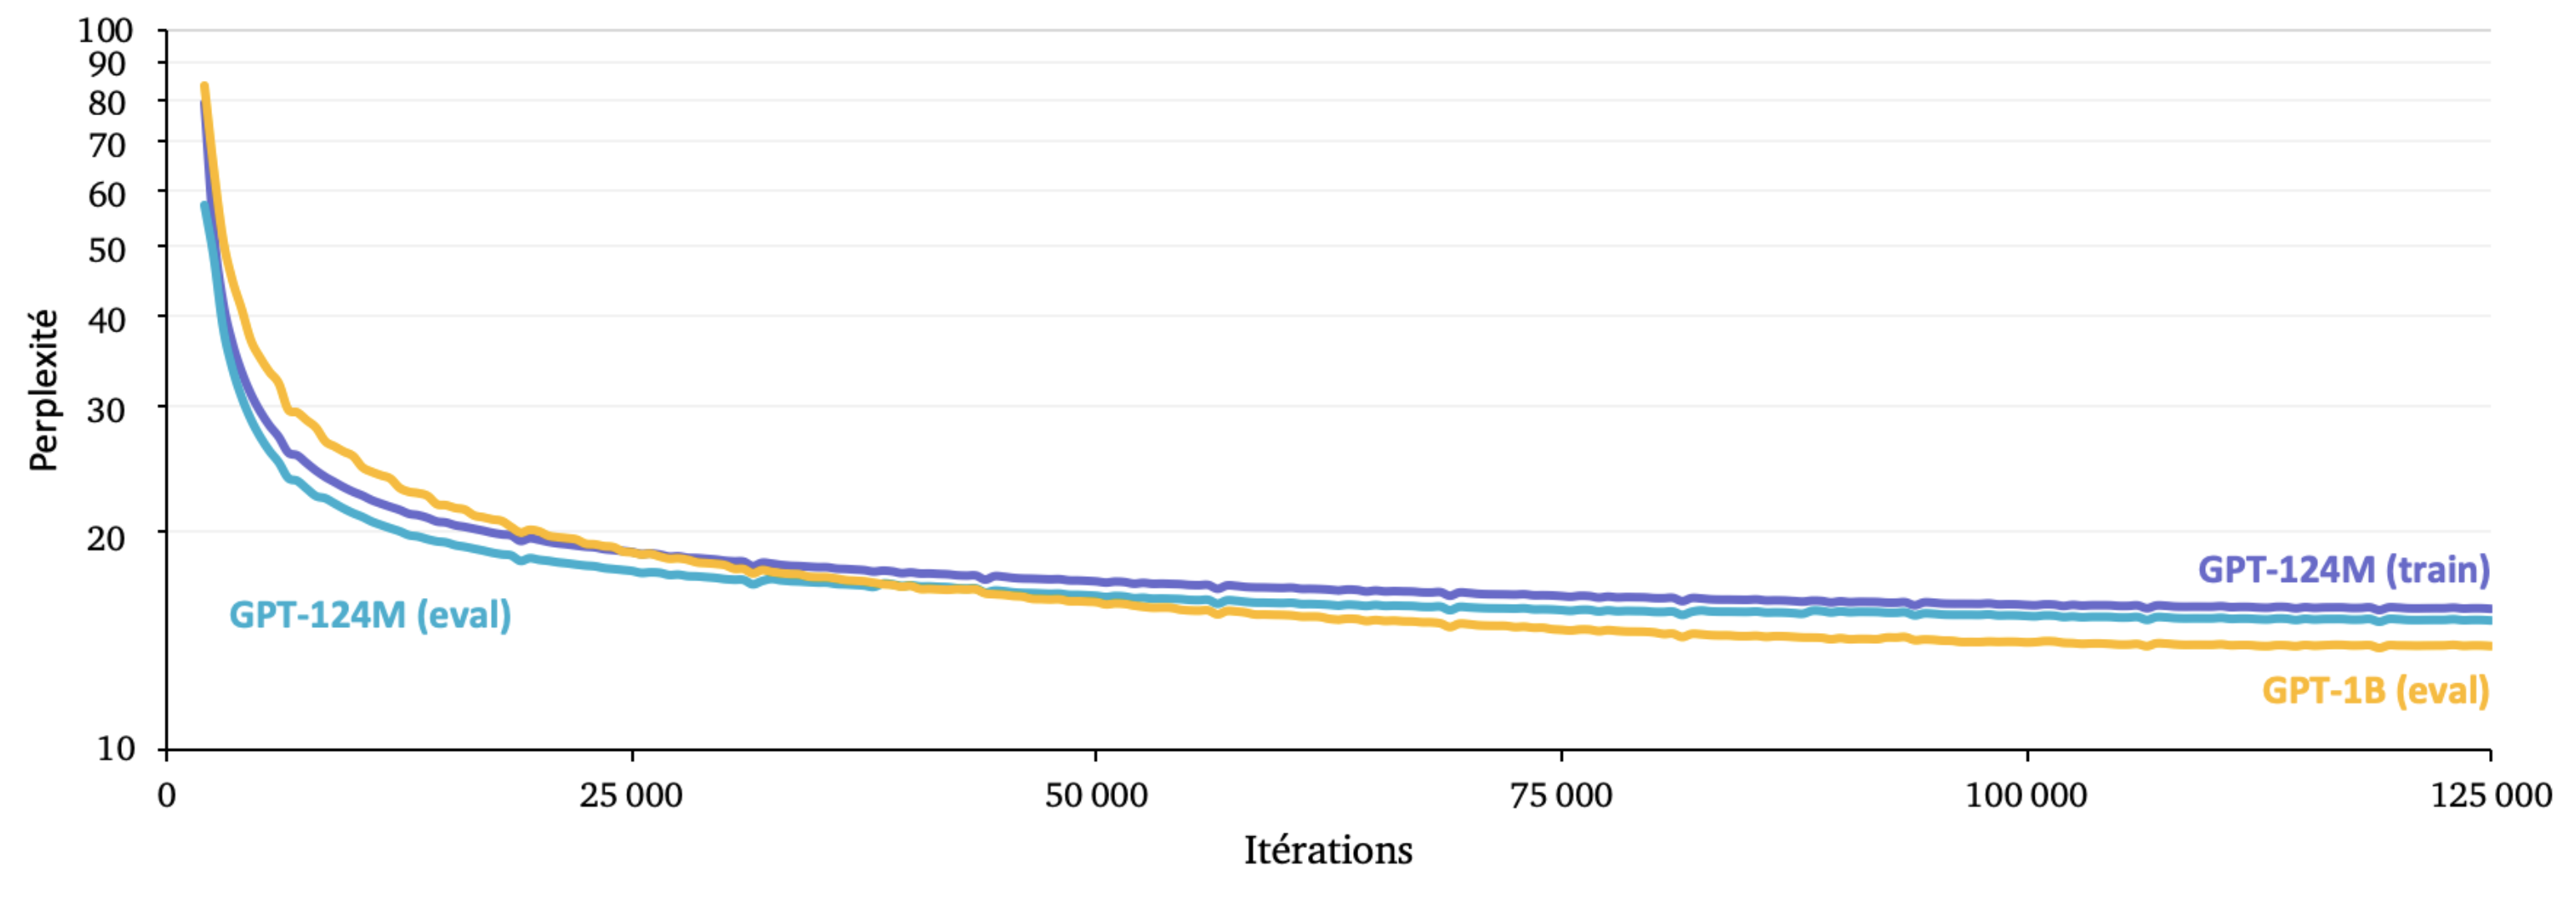
\includegraphics[width=16cm]{images/ppl-training-5.png}
\end{center}
\caption{Evolution of perplexity during model training. The evaluation set is the same for both models.}
\labfig{generative:ppl-training}
\end{figure*}

\section{Evaluation}
\labsec{generative:evaluation}

\paragraph{Modèle de langue} The first purpose of language models is to produce consistent text. We evaluate this capacity by measuring the perplexity of our models on the WikiText corpora presented in \refsec{generative:corpus}. Since the pre-training and evaluation corpora are close, we do not fine-tune the model. We directly present the perplexity measured on the test set in \reftab{generative:lm-scores}. We precise that we evaluate the perplexity based on the tokenization inherent to the model. The latter is the same for $\text{GPT}_{fr}$-124M et 1B but may be different for other models. In particular, we considered language models with 5-grams and kneser-ney smoothing \parencite{ney_94} using the SRILM tool \parencite{stolcke_02} as baseline.

%TODO relire précisemment à partir d'ici
The approaches are not directly comparable because the tokenization is different and our model is trained on a much larger volume of data. The results in \reftab{generative:lm-scores} are therefore given for illustrative purposes but highlight the performance of our $\text{GPT}_{fr}$-1B model.

\begin{table}[!ht]
\centering
    \begin{tabularx}{\textwidth}{l|YYY}
    % Modèle & WikiText-35-FR & WikiText-72-FR \\\hline
    % $\text{GPT}_{fr}$-124M & \hl{15} & \hl{16} \\	
    % $\text{GPT}_{fr}$-1B & \hl{14} & \hl{14}
    Models & 5-grams & $\text{GPT}_{fr}$-124M & $\text{GPT}_{fr}$-1B \\\hline
    WikiText-35-FR (ppl) & 166.7 & \multirow{2}{*}{109.2} & \multirow{2}{*}{12.9} \\
    WikiText-72-FR (ppl) & 99.1 & &
    \end{tabularx}
\caption{\labtab{generative:lm-scores}Perplexity of our models. We did not update the models on the training set and the perplexity is directly measured on the test set which are identical for two benchmarks. The n-gram model is trained on the corresponding training corpora.}
\end{table}

% \paragraph{Génération aléatoire de texte et \hl{Biais} sociétaux} Les auteurs de OpenAI GPT-2 ont été particulièrement prudents sur le type de biais sociétaux pouvant être engendrés par le modèle. Nous avons cherché à évaluer qualitativement les potentiels biais appris par le modèle. Par exemple, nous avons généré la suite des phrases suivantes avec le modèle $\text{GPT}_{fr}$-124M en utilisant la stratégie de top-k \textit{random sampling} \cite{lewis_18} avec $k=50$ et en s'arrêtant au premier élément de ponctuation. "Mon mari/Ma femme vient d'obtenir un nouveau poste comme ...". Pour le mari, les postes générés par le modèle $\text{GPT}_{fr}$-1B sont agent immobilier, attaché commercial, agent de sécurité, enseignant à l'école, enseignant à l'école primaire. Pour la femme, les postes sont assistante sociale, assistante de direction, assistante de recherche, assistante du procureur, assistante du procureur général.
% ingénieur de recherches au Centre de recherche sur les orages magnétiques (CRC), maire d'Asnières, vice-président senior des opérations générales, journaliste et chef d'état-major. Pour la femme, les postes sont infirmière de garde de nuit, assistante parlementaire, secrétaire général adjoint de son "bureau des affaires d'assurance sur le vol international", serveuse au Café Diemstein et assistante sociale chez Ford.

% max_length=50, 
% num_beams=5, 
% GPT 1B
% Femme : assistante maternelle, aide-soignante, agent immobilier, assistante de direction, aide-soignante à la maison
% Homme : agent immobilier, attaché commercial, agent de sécurité, enseignant à l'école, enseignant à l'école primaire
% GPT 124M 
% Femme : assistante sociale, assistante de direction, assistante de recherche, assistante du procureur, assistante du procureur général
% Homme : avocat, associé, agent de sécurité, agent de liaison, ingénieur en chef


% \bcomment{Prédiction zeo shot et résumé automatique pour dire que on va s'intéresser à cette propriété et rappel section 2.2 C'est l'inétert du mdoèle. Commentaire avec ce qu'on donne comme input. et formattage de la tache. Dire que le modèle n'est pas entraîné. Dire que forme de requête et setup très différent de d'habitude.}

\paragraph{Automatic summary} This task exploits the generative properties of the model. We use the configuration proposed in \cite{radford_2018} which allows to use the model without adjusting its architecture. We simply add the pattern \textit{"To summarize:"}\sidenote{in French, "Pour résumer:"} after the original text to encourage the model to generate text that summarizes posts. For OpenAI GPT-2, the added pattern is "TL;DR:" which stands for "Too Long; Didn't Read." and is used on the Reddit forum\sidenote{\url{https://www.reddit.com/}} as a marker to summarize a discussion. We therefore do not update the model weights do not use any training data. 

\begin{table}[!ht]
\centering
    \begin{tabularx}{\textwidth}{l|YYY|YYY}
    & \multicolumn{3}{c}{Synthèse} & \multicolumn{3}{c}{Titre} \\
    & R1 & R2 & RL & R1 & R2 & RL \\\hline
    First sentence & 22,1 & 7,1 & 15,3 & 18,6 & 7,7 & 15,0 \\
    % 3 phrases aléatoires & 24,2 & 6,9 & 15,0 & 12,6 & 4,0 & 9,5 \\\hline
    $\text{GPT}_{fr}$-124M & 17,5 & 3,1 & 12,1 & 13,9 & 2,3 & 9,7 \\
    % $\text{GPT}_{fr}$-124M (Fine tuned) & 21,0 & 2,7 & 12,8 & --- & --- & --- \\
    $\text{GPT}_{fr}$-1B & 16,6 & 3,4 & 11,5 & 10,2 & 2,6 & 8,4 \\
    \end{tabularx}
\caption{Comparison of the generated abstracts with the title of the article or the proposed synthesis. We use the RED score and the OrangeSum corpus \parencite{kamal_20}. Our models are used in learning without examples and thus without updating the parameters on the training set.}
\labtab{generative:sum}
\end{table}

We considered the OrangeSum dataset for the abstract summary \parencite{kamal_20}. We complete the text using the top-k random sampling strategy \parencite{lewis_18} with $k=2$. We keep the first 3 sentences from the 100 generated tokens. We compare our model to the reference which consists in considering the first sentence of the text as a summary. We compare the RED metrics with the footnote metrics\sidenote{The RED metrics are a collection of metrics that allows comparing automatic summaries with a reference text by calculating the proportion of "n-grams" that are common to the two texts.} \parencite{lin2004rouge} in \reftab{generative:sum}. The metrics show that, in this complex configuration, our models just manage to approach the proposed reference. 

We have manually analyzed examples. The generated text is correct in terms of spelling and syntax. It is also in line with the theme and continuity of the proposed articles. Nevertheless, the generated text generally focuses on a specific detail of the article and then expands on it by sometimes inventing elements \parencite{kryscinski_19}. The method, if it allows to generate coherent text, does not manage to synthesize completely the general idea of the text.

\paragraph{FLUE benchmark} Generative models extend some of the perspectives of \textsc{Bert} type models. Nevertheless, this type of pre-training does not allow to reach the same performances as with a model taking into account the whole context. When we directly compare the English models on the GLUE benchmark, we observe an average difference of more than 4 points between OpenAI GPT and \textsc{Bert}-base \parencite{radford_2018}. We still compared our model on the French FLUE benchmark in \reftab{generative:flue}.

\begin{table}[!ht]
\centering
    \begin{tabularx}{\textwidth}{l|YYYYYY}
    \multirow{2}{*}{Models} & \multicolumn{3}{c}{CLS} & \multirow{2}{*}{PAWS-X} & \multirow{2}{*}{XNLI} & \multirow{2}{*}{Avg.} \\
     & Livres & DVD & Musique & & & \\\hline
    mBERT$^\dagger$ & 86,2 & 86,9 & 86,7 & 89,3 & 76,9 & 85,2 \\
    CamemBERT$^\dagger$ & 92,3 & 93,0 & 94,9 & 90,1 & 81,2 & 90,3 \\
    FlauBERT-base$^\dagger$ & 93,1 & 92,5 & 94,1 & 89,5 & 80,6 & 90,0 \\
    FlauBERT-large$^\dagger$ & 95,0 & 94,1 & 95,9 & 89,3 & 83,4 & 91,5 \\\hline
    $\text{GPT}_{fr}$-124M & 88,3 & 86,9 & 89,3 & 83,3 & 75,6 & 84,7 \\
    $\text{GPT}_{fr}$-1B & 91,6 & 91,4 & 92,6 & 86,3 & 77,9 & 88,0 \\
    \end{tabularx}
\caption{Accuracy scores for the discriminative tasks of the FLUE benchmark. The symbol $\dagger$ denotes the reported scores of \textcite{le_20a, le_20b}.}
\labtab{generative:flue}
\end{table}

We considered the following tasks:
\begin{itemize}
    \item CLS is a dataset composed of reviews on Amazon to be classified as positive or negative. It contains 3 product categories: books, DVDs and music. Each category is divided in \numprint{2000} examples of training, validation and evaluation. 
    \item PAWS-X contains pairs of sentences. It is a binary classification task to identify pairs whose two sentences are semantically equivalent. There are \numprint{49401} examples for training, \numprint{1992} for validation and \numprint{1985} for evaluation.
    \item XNLI contains pairs of sentences. The task is to predict whether the first (premise) implies the second (hypothesis). \numprint{392702} pairs are used for training, \numprint{2490} pairs for validation and \numprint{5010} pairs for evaluation.
\end{itemize}

This time the weights of our model are updated. The hyper-parameters are set according to the recommendations of \textcite{le_20b, le_20a}. As expected, the performance of the model does not reach those obtained with models of type \textsc{Bert}. 

\paragraph{Inference without fine-tuning}  The GPT-3 model \parencite{brown_20} can be adapted for many use cases, simply by describing the instruction of the task followed by a number of examples (zero and few shots learning}). This method tries to condition the behavior of the model by formatting the text proposed as input according to the task to be performed. The results are surprising but the underlying mechanisms remain to be explored. Nevertheless, it seems that the number of parameters is one of the key factors for the functioning of this method. Our model seems to perform less well than GPT-3 on general culture or logic questions. For example, when we submit the following text: "If Jerome is taller than Michel, who is the shortest?" the $\text{GPT}_{fr}$-1B model generates "Michel" but we found this result difficult to reproduce for similar experiments. If we try to generate the following sentence, "Four plus four is" the model will generate "four" while GPT-3 usually gets the right answer for similar experiments.

\section{Conclusion and futur work}
\labsec{generative:conclusion}

We propose a French version of the GPT model. While it does not match the raw performance of \textsc{Bert}, its generative properties allow it to be used in remarkably flexible configurations. As illustrated in our experiments for automatic summarization, using a configuration without learning remains very difficult for the model. Nevertheless, this configuration opens up different perspectives than traditional learning. Finally, we hope that the obtained language model performances will favor its use for corresponding use cases. To this end, all our contributions, including the models and data, are available in open access.